
\let\negmedspace\undefined
\let\negthickspace\undefined
\documentclass[journal]{IEEEtran}
\usepackage[a5paper, margin=10mm, onecolumn]{geometry}
%\usepackage{lmodern} % Ensure lmodern is loaded for pdflatex
\usepackage{tfrupee} % Include tfrupee package

\setlength{\headheight}{1cm} % Set the height of the header box
\setlength{\headsep}{0mm}     % Set the distance between the header box and the top of the text

\usepackage{gvv-book}
\usepackage{gvv}
\usepackage{cite}
\usepackage{amsmath,amssymb,amsfonts,amsthm}
\usepackage{algorithmic}
\usepackage{graphicx}
\usepackage{textcomp}
\usepackage{xcolor}
\usepackage{txfonts}
\usepackage{listings}
\usepackage{enumitem}
\usepackage{mathtools}
\usepackage{gensymb}
\usepackage{comment}
\usepackage[breaklinks=true]{hyperref}
\usepackage{tkz-euclide} 
\usepackage{listings}
% \usepackage{gvv}                                        
\def\inputGnumericTable{}                                 
\usepackage[latin1]{inputenc}                                
\usepackage{color}                                            
\usepackage{array}                                            
\usepackage{longtable}                                       
\usepackage{calc}                                             
\usepackage{multirow}                                         
\usepackage{hhline}                                           
\usepackage{ifthen}                                           
\usepackage{lscape}
\begin{document}

\bibliographystyle{IEEEtran}
\vspace{3cm}

\title{NCERT-10.4.4.1.2}
\author{EE24BTECH11023 - RASAGNA}

% \maketitle
% \newpage
% \bigskip
{\let\newpage\relax\maketitle}

\renewcommand{\thefigure}{\theenumi}
\renewcommand{\thetable}{\theenumi}
\setlength{\intextsep}{10pt} % Space between text and floats


\numberwithin{equation}{enumi}
\numberwithin{figure}{enumi}
\renewcommand{\thetable}{\theenumi}
\textbf{Question:}
Find the nature of the roots of the following quadratic equation. If the real roots exist,find them:
\begin{align*}
    3x^2-4{\sqrt{3}}x+4=0
\end{align*}
\textbf{Theoritical Solution:}
The standard quadratic equation is:
\begin{align}
    ax^2 + bx + c = 0
\end{align}
Here, \( a = 3, b = -4{\sqrt{3}}, c = 4 \).
Computing the value of determinant,
\begin{align}
    \triangle =b^2-4ac
\end{align}
\begin{align}
    \triangle =(-4{\sqrt{3}})^2-4(3)(4)
\end{align}
\begin{align}
    \therefore \triangle =0
\end{align}
$\therefore$ The given equation has two equal and real roots.\\
The roots are given by:
\begin{align}
    x = \frac{-b \pm \sqrt{b^2 - 4ac}}{2a}
\end{align}
Substitute the values of \( a, b, \) and \( c \):
\begin{align}
   & x = \frac{-(-4{\sqrt{3}}) \pm \sqrt{(-4{\sqrt{3}})^2 - 4(3)(4)}}{2(3)} \\
   & = \frac{2}{\sqrt{3}}
\end{align}
Thus, the roots of the equation are:
\begin{align}
x_1=x_2=\frac{2}{\sqrt{3}}
\end{align}
\textbf{Computational Solution}\\
We use fixed point iteration method to find the roots,\\
From the equation we can reformulate it as \\
\begin{align}
    g(x)=\frac{\sqrt{4{\sqrt{3}}x-4}}{\sqrt{3}}
\end{align}
Now let us assume the initial guess of x as $x_0=2$
Use the iterative formula,
\begin{align}
    x_{n+1}=g(x_n)
\end{align}
 Repeat the iterations until the sequence ${x_{n+1}}$ converges to a fixed point.
 Convergence is often checked using
A predefined tolerance $\epsilon$ where $|x_{n+1}-x_n|<\epsilon$ or maximum number of iterations.
The result obtained by computational approach is :\\
Root 1 = 1.154701 + 0.000000i\\
Root 2 = 1.154701 - 0.000000i
\begin{center}
    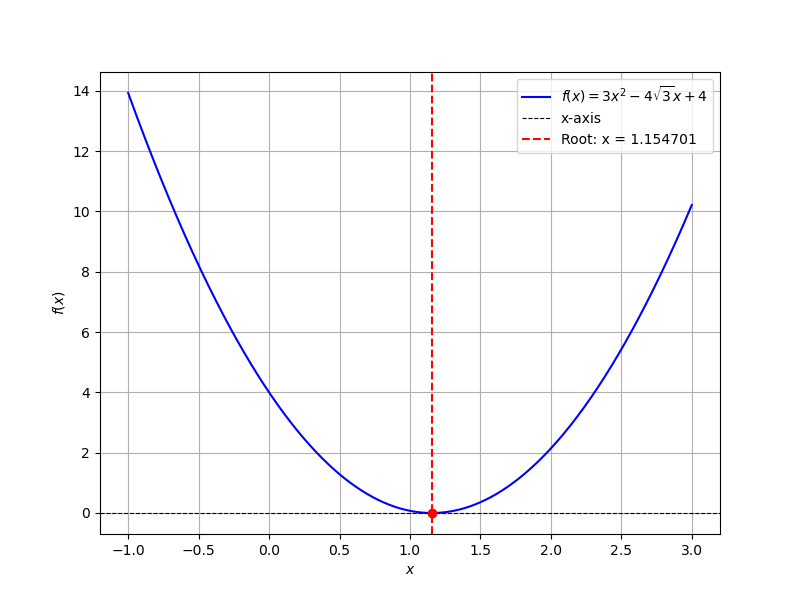
\includegraphics[width=0.75\columnwidth]{figs/eq.png}
\end{center}

\end{document}